% ============================================================================
% SEC01.TEX - Section 3.1: MonoBehaviour dan Struktur Skrip
% ============================================================================

\section{MonoBehaviour dan Struktur Skrip}

\begin{learningoutcomes}
\item Memahami konsep MonoBehaviour
\item Mampu membuat skrip C\# pertama di Unity
\item Memahami struktur dasar skrip Unity
\item Mampu melampirkan skrip ke GameObject
\end{learningoutcomes}

\subsection{Pengertian MonoBehaviour}

\begin{definisi}[MonoBehaviour]
MonoBehaviour adalah kelas dasar untuk skrip Unity yang memungkinkannya melekat pada GameObject dan berinteraksi dengan Unity Engine \cite{UnityScriptingAPI2024}.
\end{definisi}

\subsection{Struktur Dasar Skrip Unity}

\begin{figure}[ht]
    \centering
    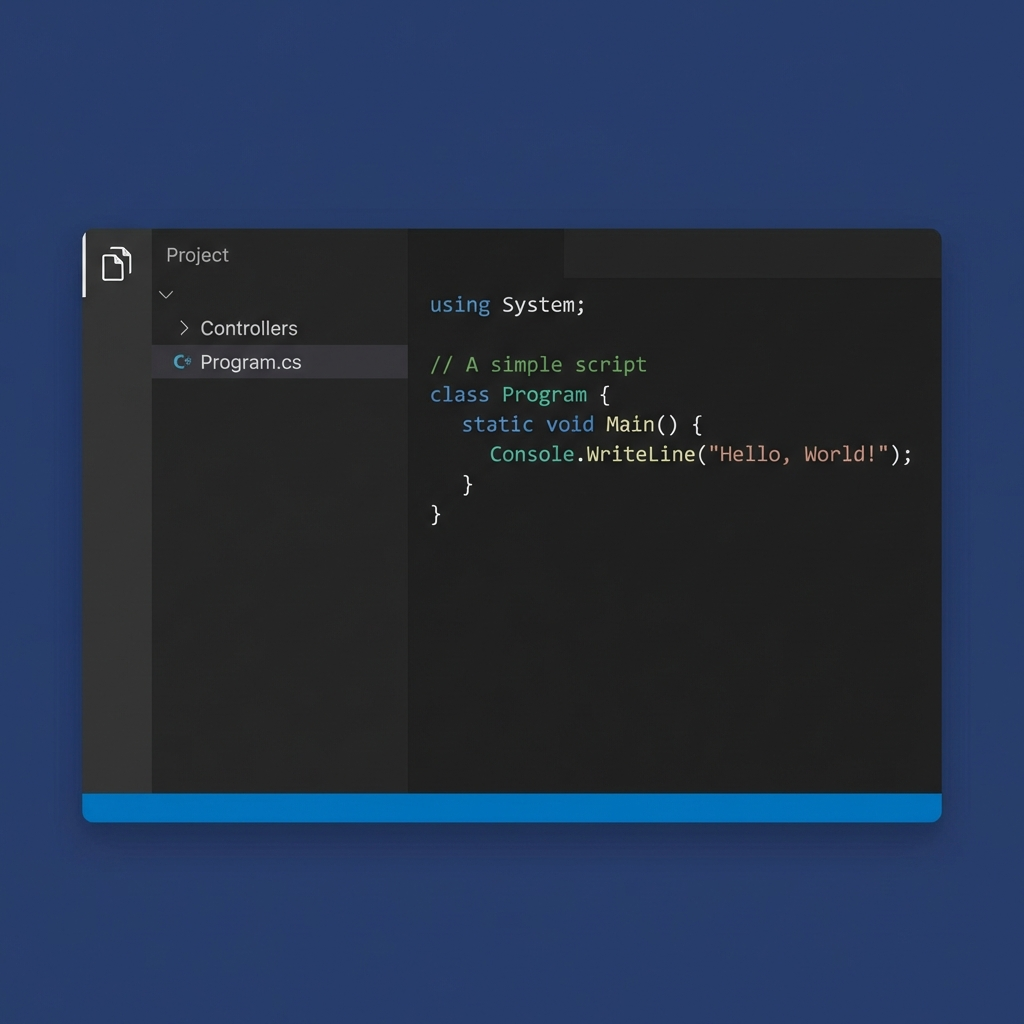
\includegraphics[width=0.8\textwidth]{figures/vscode.png}
    \caption{Ilustrasi Code Editor (Visual Studio Code)}
    \label{fig:vscode}
\end{figure}

\begin{lstlisting}[language={[Sharp]C}, caption=Contoh Skrip Unity Dasar]
using UnityEngine;

public class PlayerController : MonoBehaviour
{
    // Variabel
    public float speed = 5f;
    
    // Lifecycle functions
    void Start()
    {
        Debug.Log("Player Controller Started");
    }
    
    void Update()
    {
        // Code yang dijalankan setiap frame
    }
}
\end{lstlisting}

\subsection{Melampirkan Skrip ke GameObject}

\begin{enumerate}
\item Buat skrip di Project window
\item Drag skrip ke GameObject di Hierarchy
\item Atau pilih GameObject, klik "Add Component", cari skrip
\end{enumerate}

\begin{catatan}
Semua skrip Unity harus inherit dari MonoBehaviour untuk dapat berfungsi dengan Unity Engine.
\end{catatan}
